%=======================================================================
% cap4_datos.tex — Levantamiento de datos
%=======================================================================

Este capítulo documenta las fases de comprensión y preparación de los datos:
cómo se definió el conjunto de especies, cómo se construyeron los tres corpus
del sistema (audio, imagen y avistamientos con covariables ambientales), qué
decisiones se tomaron durante el levantamiento y en qué se apartó la
implementación del plan original.

%-----------------------------------------------------------------------
\section{Repositorio reproducible y acceso a las fuentes}\label{sec:repositorio}

El levantamiento se implementó como una secuencia de \textit{scripts}
numerados sobre un paquete Python (\texttt{biomonitor}) con módulos de
datos, audio, visión, fusión multimodal y distribución de especies. Las
dependencias se fijan con \texttt{uv} y Python 3.12, los hiperparámetros
viven en un único archivo de configuración y las credenciales se cargan
desde variables de entorno. Las descargas y los entrenamientos se ejecutaron
en un Mac con procesador Apple M4 Pro, con aceleración por GPU mediante
Metal/MPS. El código, la configuración y los \textit{scripts} están
publicados en \url{\repoURL}.

Las fuentes se consultan mediante sus interfaces programáticas: la API v3 de
Xeno-canto, la API pública de GBIF para fotografías y registros de
ocurrencia, y Google Earth Engine (GEE) para las covariables ambientales. El
listado del RCE se descarga directamente del sitio del Ministerio del Medio
Ambiente. Los modelos preentrenados provienen de los repositorios abiertos
\texttt{timm} y Hugging Face.

%-----------------------------------------------------------------------
\section{Conjunto de especies objetivo}\label{sec:especies}

El conjunto objetivo se construyó a partir del listado oficial del
Reglamento de Clasificación de Especies (RCE), que asigna a cada especie
evaluada una categoría de conservación. La \tabref{tab:rce} resume las
categorías que aparecen en este trabajo y la \figref{fig:seleccion} muestra
el proceso de selección completo.

\begin{table}[!htb]
  \centering\small
  \caption{Categorías de conservación del RCE que aparecen en este trabajo y
  número de especies del conjunto objetivo en cada una.}
  \label{tab:rce}
  \begin{tabular}{@{}l l l r@{}}
    \toprule
    Sigla & Categoría & Significado & Especies \\
    \midrule
    CR & En Peligro Crítico & riesgo extremadamente alto de extinción & 1 \\
    EN & En Peligro & riesgo muy alto de extinción & 5 \\
    VU & Vulnerable & riesgo alto de extinción & 7 \\
    NT & Casi Amenazada & cerca de calificar como amenazada & 1 \\
    LC & Preocupación Menor & evaluada y sin riesgo actual & 3 \\
    NE & No Evaluada & sin evaluación formal en el RCE & 38 \\
    \bottomrule
  \end{tabular}
\end{table}

\begin{figure}[!htb]
  \centering
  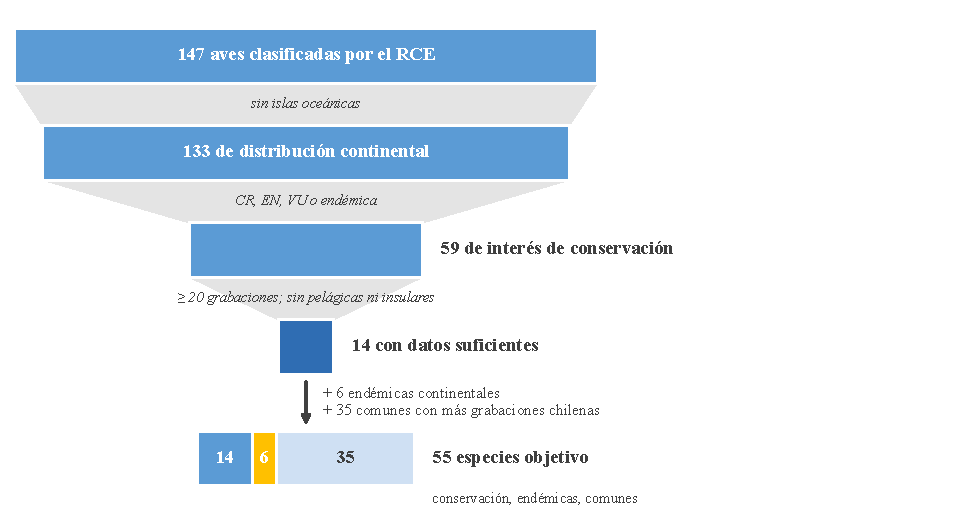
\includegraphics[width=\textwidth]{fig_seleccion_especies}
  \caption{Construcción del conjunto de 55 especies objetivo: de las 147
  aves clasificadas por el RCE se conservan las de distribución continental,
  luego las de interés de conservación y por último las que tienen datos
  suficientes; a esas 14 se suman 6 endémicas y 35 comunes.}
  \label{fig:seleccion}
\end{figure}

El punto de partida son las 147 aves clasificadas por el RCE. Primero se
filtraron las de distribución continental (133) y, entre ellas, las de
interés de conservación (CR, EN o VU, o endémicas de Chile), lo que dejó 59
candidatas. Para cada una se realizó un censo de datos: grabaciones en
Xeno-canto (globales y con localidad en Chile) y fotografías con grado de
investigación en GBIF. Se descartaron las especies pelágicas (aves marinas
que viven en mar abierto, como albatros, petreles y pingüinos) e insulares
(restringidas a las islas oceánicas), cuyo monitoreo responde a otra lógica,
y las que no alcanzaban un mínimo de 20 grabaciones a nivel global. Quedaron
14 especies de interés de conservación: una CR (\textit{Podiceps
gallardoi}), cinco EN, siete VU y el choroy (\textit{Enicognathus
leptorhynchus}), endémico en Preocupación Menor. Segundo, se agregaron las
seis especies endémicas continentales restantes con grabaciones suficientes
(tenca, chiricoca, turca, hued-hued castaño, tapaculo y churrín del norte).
Tercero, se completó el conjunto con las 35 especies comunes con mayor
número de grabaciones chilenas en Xeno-canto, que aportan masa de
entrenamiento y representan los principales ecosistemas del país. En el
resto del documento las especies se agrupan en tres categorías:
\emph{amenazadas} (13 especies CR, EN o VU), \emph{endémicas} no amenazadas
(7, incluido el choroy) y \emph{comunes} (35). El listado completo se
presenta en el Apéndice~\ref{ape:especies}.


La exclusión de las pelágicas no es solo una decisión de datos. Cerca de 25
de las 59 candidatas lo son, apenas vocalizan en tierra y su distribución es
oceánica, incompatible con un modelo de distribución terrestre basado en
vegetación y clima. La consecuencia es que no es posible reunir 50 especies
únicamente con aves amenazadas, lo que obligó a completar el conjunto con
especies comunes. La propuesta original pedía ``foco'' en las amenazadas, no
exclusividad, y esa composición preserva el foco con una base de
entrenamiento suficiente.

%-----------------------------------------------------------------------
\section{Corpus de audio}\label{sec:corpus-audio}

\subsection{Censo y disponibilidad}

El censo identificó \num{2587} grabaciones de Xeno-canto con localidad en
Chile para las 55 especies. La \tabref{tab:corpus-grupos} resume la
disponibilidad por grupo y la \figref{fig:corpus} la detalla por especie. La
asimetría es fuerte. Las 13 especies amenazadas reúnen 129 grabaciones
chilenas, el \SI{5}{\percent} del total, con una mediana de 6 por especie, y
cuatro de ellas no tienen ninguna. Las 35 comunes concentran el
\SI{81}{\percent}. La especie más grabada (\textit{Turdus falcklandii}, 186)
tiene por sí sola más audio que las 13 amenazadas juntas.

\begin{table}[!htb]
  \centering\small
  \caption{Grabaciones de Xeno-canto con localidad en Chile por grupo de
  especies del conjunto objetivo.}
  \label{tab:corpus-grupos}
  \fitwidth{\begin{tabular}{@{}l r r r r r r@{}}
    \toprule
    Grupo & Especies & Grabaciones & \% del total & Mínimo & Mediana & Máximo \\
    \midrule
    Amenazadas (CR, EN, VU) & 13 & 129 & 5,0 & 0 & 6 & 34 \\
    Endémicas (incl.\ choroy) & 7 & 355 & 13,7 & 34 & 46 & 86 \\
    Comunes & 35 & \num{2103} & 81,3 & 32 & 51 & 186 \\
    \midrule
    Total & 55 & \num{2587} & 100 & 0 & 44 & 186 \\
    \bottomrule
  \end{tabular}}
\end{table}

\begin{figure}[!htb]
  \centering
  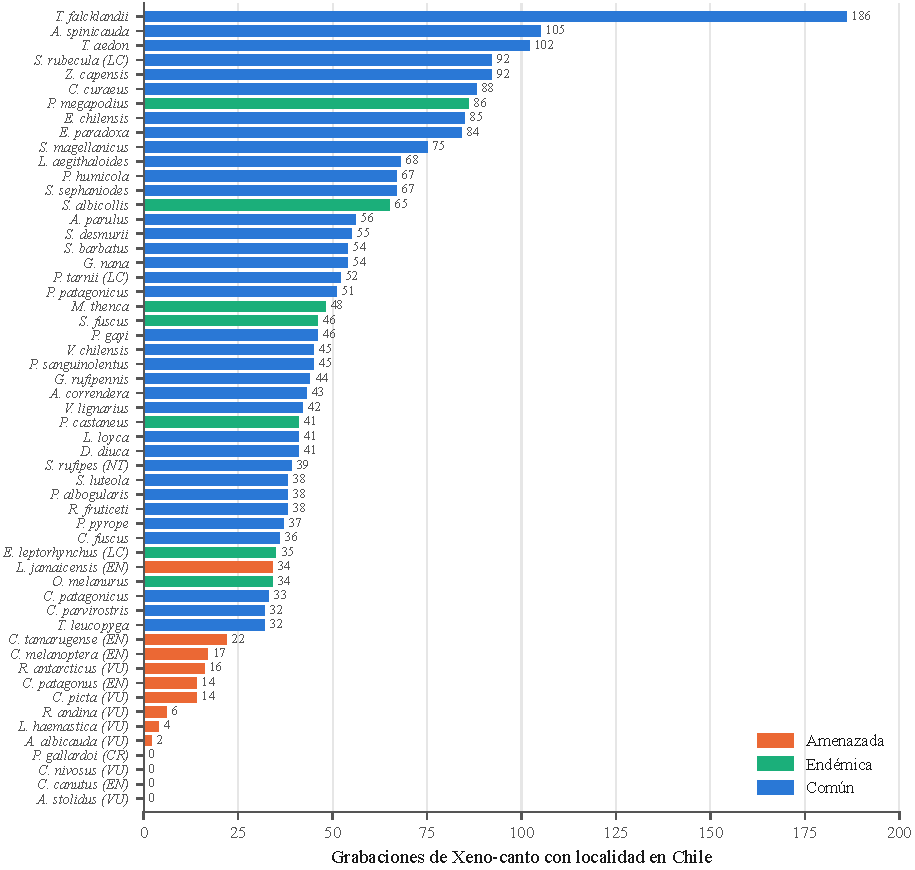
\includegraphics[width=0.95\textwidth]{fig_corpus_especies}
  \caption{Grabaciones de Xeno-canto con localidad en Chile por especie del
  conjunto objetivo, coloreadas por grupo. Entre paréntesis, la categoría del
  RCE cuando la especie ha sido evaluada.}
  \label{fig:corpus}
\end{figure}

\subsection{Descarga y composición del corpus}

Dado el censo anterior, el corpus de entrenamiento no se limitó a Chile. Para
cada especie se descargaron hasta 50 grabaciones de calidad A, B o C y de
menos de cuatro minutos, priorizando las de localidad chilena y completando
con grabaciones de otros países cuando faltaban. La calidad es la que asignan
los propios usuarios de Xeno-canto en una escala de A (grabación nítida, con
el ave en primer plano y casi sin ruido) a E (apenas audible). Se conservaron
las tres mejores. Dos razones justifican el uso de audio extranjero. La
primera es acústica: la firma vocal es específica de la especie y, para aves
de distribución amplia, las poblaciones vecinas comparten el repertorio. La
segunda es práctica: sin grabaciones externas, las cuatro especies
amenazadas sin audio chileno quedarían fuera del clasificador. El tope de 50
por especie acota el desbalance, pues las comunes tendrían hasta 186. La
\tabref{tab:corpus-audio} resume el corpus resultante y la
\figref{fig:datos-especie} muestra su composición por especie y origen.

\begin{figure}[p]
  \centering
  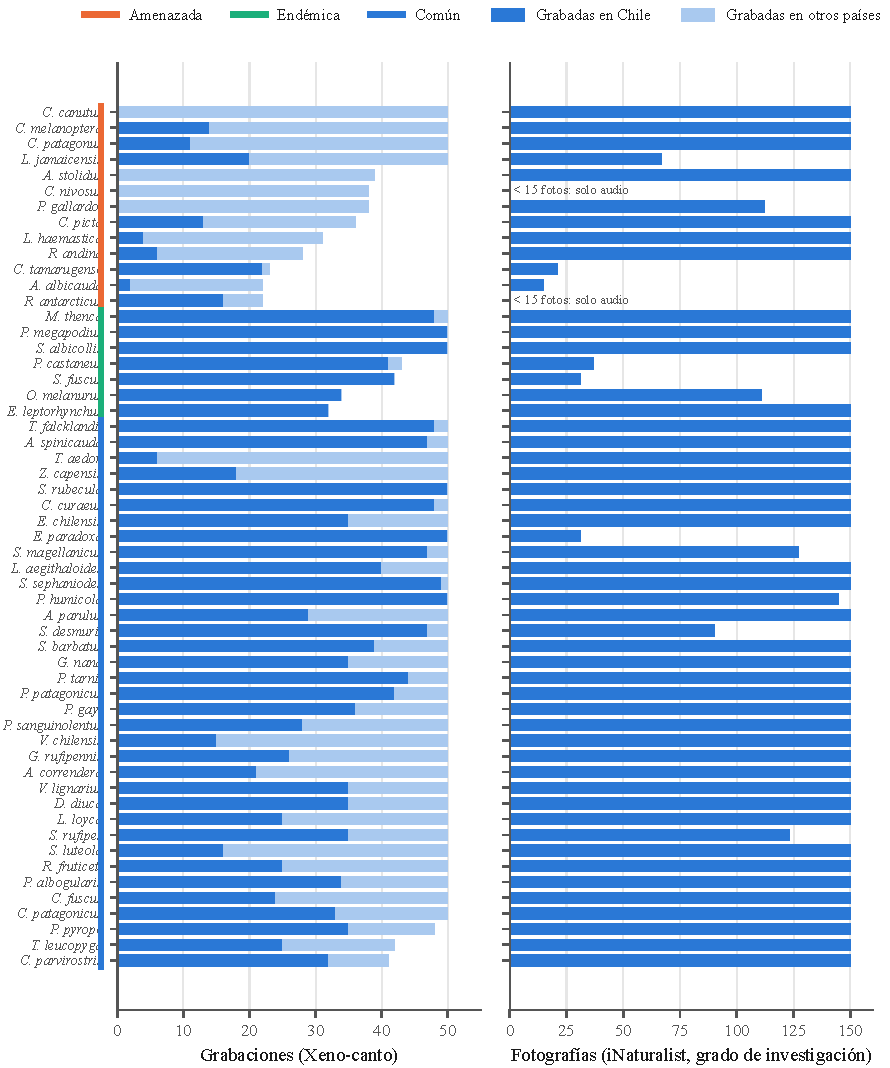
\includegraphics[width=0.88\textwidth]{fig_datos_por_especie}
  \caption{Composición de los corpus por especie; las especies se ordenan por grupo
  de conservación (franja de color) y número de grabaciones. Izquierda:
  grabaciones de audio del corpus de entrenamiento según su origen.
  Derecha: fotografías con grado de investigación de iNaturalist. Las dos
  especies con menos de 15 fotografías no participan del clasificador de
  imagen.}
  \label{fig:datos-especie}
\end{figure}

\begin{table}[!htb]
  \centering\small
  \caption{Corpus de audio descargado y preprocesado.}
  \label{tab:corpus-audio}
  \begin{tabularx}{\textwidth}{@{}l X@{}}
    \toprule
    Característica & Valor \\
    \midrule
    Grabaciones & \num{2509} seleccionadas; \num{2508} decodificadas correctamente (una corrupta) \\
    Duración total & \SI{25,6}{\hour} (mediana \SI{24}{\second} por grabación; \SI{7}{\percent} dura \SI{5}{\second} o menos) \\
    Grabaciones por especie & mínimo 22 (\textit{Agriornis albicauda}, \textit{Rallus antarcticus}), tope 50; 39 especies alcanzan el tope \\
    Origen & \SI{64}{\percent} Chile (\num{1609}); \SI{36}{\percent} de otros 36 países (Argentina 434, Brasil 77, Ecuador 56, Perú 45, Estados Unidos 44) \\
    Especies con menos de la mitad de audio chileno & 17; cuatro sin ninguna grabación chilena (\textit{P.~gallardoi}, \textit{C.~canutus}, \textit{C.~nivosus}, \textit{A.~stolidus}) \\
    Calidad de la grabación (escala de Xeno-canto) & A \SI{69}{\percent}, B \SI{26}{\percent}, C \SI{4}{\percent} \\
    Tipo de vocalización & canto en el \SI{47}{\percent} de las grabaciones, llamado en el \SI{56}{\percent} (categorías no excluyentes) \\
    Particiones (grabaciones) & entrenamiento \num{1721} (\SI{69}{\percent}), validación 394 (\SI{16}{\percent}), prueba 393 (\SI{16}{\percent}) \\
    \bottomrule
  \end{tabularx}
\end{table}

\subsection{Preprocesamiento y particiones}

Cada archivo se decodificó, se convirtió a mono, se remuestreó a
\SI{32}{\kilo\hertz} y se almacenó en una caché comprimida sin pérdida
junto a un manifiesto con sus metadatos (especie, identificador de
Xeno-canto, duración, país, calidad y tipo de vocalización). Las particiones
de entrenamiento, validación y prueba (70/15/15) se construyeron a nivel de
\emph{grabación}, estratificadas por especie y con semilla fija, de modo que
todas las ventanas extraídas de un mismo archivo pertenecen a una única
partición. Las 55 especies están presentes en las tres
particiones. El conjunto de prueba tiene entre 3 (\textit{A.~albicauda}) y 8
grabaciones por especie, lo que, como se verá en el
\capref{cap:resultados}, hace ruidosas las métricas de las especies raras.

%-----------------------------------------------------------------------
\section{Corpus de imagen}\label{sec:corpus-imagen}

Las fotografías provienen de observaciones de iNaturalist con grado de
investigación, es decir, geolocalizadas y con la identificación validada por
la comunidad. Se descargaron a través de la API de GBIF \citep{inat2026gbif}
con un tope de 150 por especie. La descarga exigió dos ajustes. Primero, un
mapa de sinónimos taxonómicos: iNaturalist clasifica al fío-fío como
\textit{Elaenia albiceps} y escribe \textit{Sylviorthorhynchus desmursii}
para el colilarga, por lo que las consultas con los nombres del RCE
devolvían cero resultados. Segundo, un respaldo filtrado para las especies
con pocas fotografías: al ampliar la búsqueda a todo GBIF aparecían
espectrogramas de Xeno-canto y fotografías de especímenes de museo, de modo
que se restringió a observaciones humanas de aves vivas.

Se obtuvieron \num{7068} fotografías para las 55 especies. Dos especies
amenazadas no alcanzaron el mínimo de 15 fotografías de aves vivas
(\textit{Charadrius nivosus}, con 2, y \textit{Rallus antarcticus}, con 6)
y quedaron fuera del clasificador de imagen como especies \emph{solo audio},
que la fusión multimodal sigue cubriendo. El corpus del clasificador tiene,
por tanto, \num{7060} fotografías de 53 especies, entre 15
(\textit{A.~albicauda}) y 150 por especie, con solo dos especies bajo 30. El
\SI{52}{\percent} de las fotografías fue tomado en Chile y el
\SI{33}{\percent} en Argentina. Como cada fotografía es una observación
independiente, la partición se hizo a nivel de fotografía, estratificada por
especie y con la misma semilla: \num{4980} para entrenamiento, \num{1040}
para validación y \num{1040} para prueba. El mismo patrón de escasez del
audio reaparece aquí: las especies de mayor interés de conservación son las
que tienen menos ejemplos y conjuntos de prueba de 2 a 5 fotografías.

%-----------------------------------------------------------------------
\section{Avistamientos y covariables ambientales}\label{sec:datos-sdm}

\subsection{Registros de presencia}

Los registros de presencia para el modelo de distribución se obtuvieron de la
búsqueda pública de ocurrencias de GBIF, que agrega las observaciones de
eBird \citep{ebird2026gbif} e iNaturalist, con un tope de \num{2000} registros
por especie dentro de Chile continental (coordenadas válidas y dentro del
rectángulo de latitud \SIrange{-56}{-17,5}{\degree} y longitud
\SIrange{-75,7}{-66,4}{\degree}, que excluye las islas oceánicas). El plan
original contemplaba la base histórica de eBird (EBD), que entrega listas
completas con el esfuerzo de observación. La solicitud de acceso se envió en
julio de 2026 y, al momento de escribir este informe (octubre de 2026), no
ha sido aprobada, de modo que se optó por GBIF, que es inmediato y
reproducible. El costo de esta decisión es la pérdida del esfuerzo de
observación, que se compensa en la generación de pseudoausencias
(\secref{sec:pseudoausencias}).

Se reunieron \num{100270} registros de las 55 especies. Cuarenta y nueve
especies alcanzan el tope y cinco quedan por debajo de 500 (\textit{Anous
stolidus} tiene solo 5 y no se modela). La \figref{fig:avistamientos}
muestra su distribución. Espacialmente, siguen la geografía del esfuerzo de
observación, concentrados en la zona central y en torno a las ciudades y
rutas, y el patrón apenas cambia entre verano e invierno. Temporalmente, el
\SI{87}{\percent} corresponde a 2024--2026, por el crecimiento reciente de la
ciencia ciudadana y porque el tope por especie favorece los registros más
recientes. Estacionalmente, la mitad (\SI{51}{\percent}) se concentra en enero
y febrero, el verano austral. Esta estacionalidad mezcla la fenología de
las aves con el esfuerzo de los observadores y es una de las limitaciones
que se discuten en el \capref{cap:conclusiones}.

\begin{figure}[!htb]
  \centering
  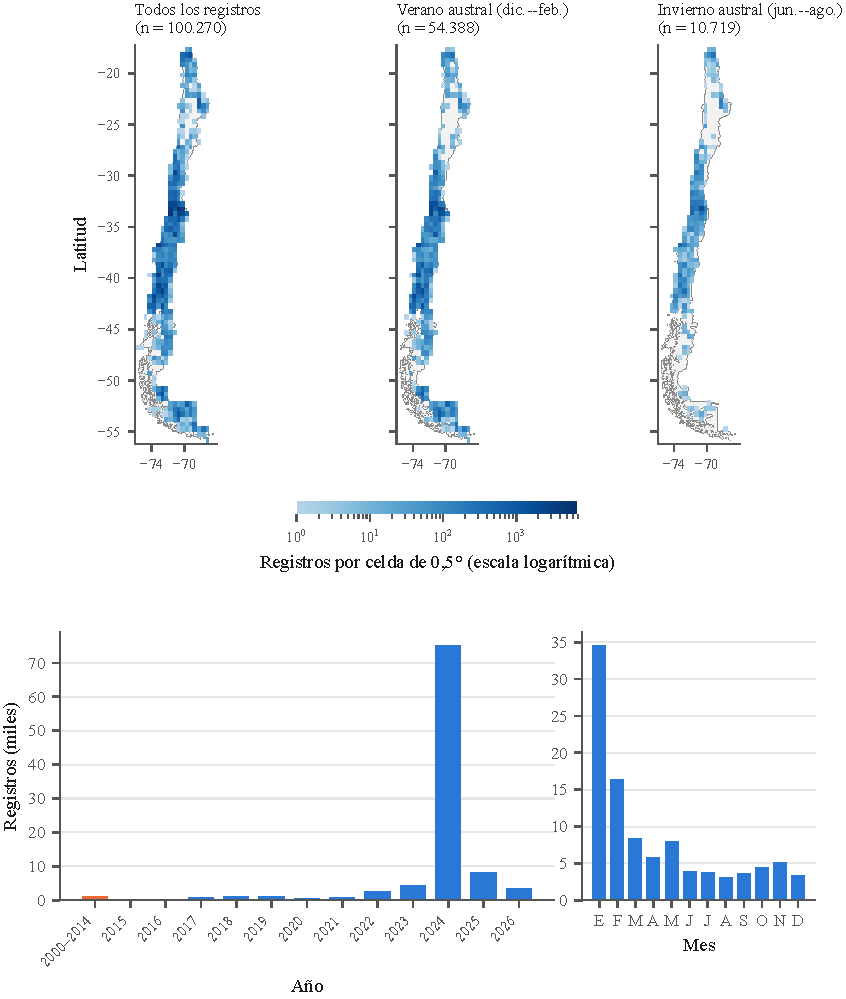
\includegraphics[width=0.92\textwidth]{fig_avistamientos}
  \caption{Registros de presencia obtenidos de GBIF (eBird e iNaturalist) para
  las 55 especies. Arriba: densidad espacial en celdas de \SI{0,5}{\degree}
  para todos los registros, para el verano y para el invierno austral.
  Abajo: distribución por año y por mes.}
  \label{fig:avistamientos}
\end{figure}

\subsection{Pseudoausencias y conjunto de datos del SDM}\label{sec:pseudoausencias}

Un modelo de distribución necesita contrastar los lugares donde la especie
está con lugares donde no está. Los registros de ciencia ciudadana solo
dicen dónde se la vio, nunca dónde se la buscó sin éxito, así que las
``ausencias'' deben construirse artificialmente: son las
\emph{pseudoausencias} o puntos de fondo (\secref{sec:teoria-sdm}). La
forma más simple, repartirlas al azar por todo el territorio, tiene un
problema: los avistamientos se concentran donde hay observadores, de modo
que el modelo aprendería a distinguir ``lugares con gente'' de ``lugares sin
gente'' en vez de hábitat bueno y malo. Para evitarlo se usó el método del
\emph{grupo objetivo} \citep{phillips2009bias}: se tomó una única muestra
aleatoria de \num{10000} avistamientos de todas las especies del conjunto,
compartida entre todas las especies modeladas, que por construcción
reproduce los lugares y meses en que la gente observa aves; cada modelo usa
\num{1500} de esos puntos como fondo (Apéndice~\ref{ape:hiperparametros}).
Así, el contraste que aprende el modelo es entre los sitios donde se vio a
la especie y los sitios comparables donde se observan aves en general. Las
presencias se limitaron a 500 registros por especie para reducir el peso de
las zonas sobremuestreadas. Tras muestrear las covariables, el conjunto de
datos quedó en \num{34926} puntos: \num{25171} presencias de 55 especies (54
con al menos 20, el mínimo para modelar) y \num{9755} puntos de fondo (los
245 restantes cayeron sobre agua o sin datos).

\subsection{Covariables ambientales}\label{sec:covariables}

Cada punto (presencia o pseudoausencia) se describe con cuatro variables
ambientales y el mes del registro (\tabref{tab:covariables},
\figref{fig:covariables}). Las variables ambientales se obtuvieron de
Google Earth Engine, una plataforma de Google que almacena en la nube
catálogos de imágenes satelitales y capas climáticas y permite consultarlos
sin descargarlos \citep{gorelick2017gee}. Para cada punto se pidió, en una
sola consulta, el valor de las cuatro capas a \SI{1}{\kilo\metre} de
resolución. El NDVI (índice de vegetación de diferencia normalizada) mide la
cantidad de vegetación verde a partir de la luz que refleja la superficie y
proviene de MODIS, un sensor de los satélites Terra y Aqua de la NASA que
observa toda la Tierra cada uno o dos días. La temperatura media anual y la
precipitación anual provienen de WorldClim, una climatología global
interpolada a partir de estaciones meteorológicas. La elevación proviene del
modelo digital de terreno SRTM. El mes del avistamiento se codifica de forma
cíclica (seno y coseno), lo que aporta el eje temporal al modelo.

\begin{figure}[!htb]
  \centering
  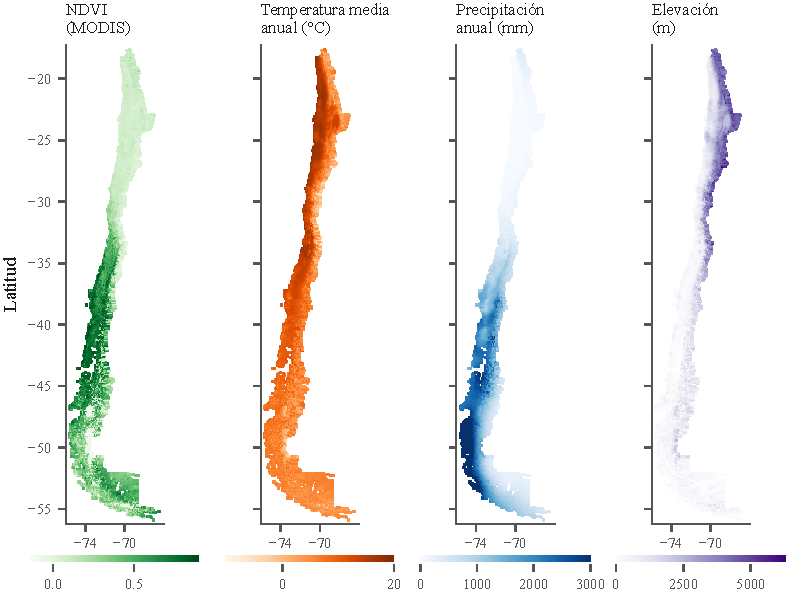
\includegraphics[width=0.9\textwidth]{fig_covariables}
  \caption{Covariables ambientales sobre la grilla de \SI{0,1}{\degree} de
  Chile continental: NDVI, temperatura media anual, precipitación anual
  (escala truncada en \SI{3000}{\milli\metre}) y elevación.}
  \label{fig:covariables}
\end{figure}

El plan original usaba el reanálisis climático ERA5 y el NDVI mensual de
Sentinel-2. Ambos se descartaron por una restricción de cómputo de la
plataforma: calcular la mediana de miles de imágenes de Sentinel-2 o el
promedio de 120 meses de ERA5 en decenas de miles de puntos excede el tiempo
máximo que Google Earth Engine permite por consulta. Se reemplazaron por
capas precalculadas, que son además el estándar en modelado de distribución
\citep{hijmans2005worldclim}. Para los experimentos con información satelital
se extrajeron también parches de cobertura de suelo de ESA WorldCover
\citep{zanaga2021worldcover} y el \textit{embedding} satelital anual de 64
dimensiones de Google (AlphaEarth Foundations, \citealp{brown2025alphaearth}).
Este \textit{embedding} es una representación numérica de cada píxel,
aprendida por un modelo de fundación a partir de múltiples satélites, y se
usó en su versión fija (2023) y pareada al año de cada observación
(2017--2025). Para dibujar mapas de
distribución se muestrearon las mismas covariables en una grilla regular de
\SI{0,1}{\degree} (\num{7910} celdas dentro de Chile continental).

\begin{table}[!htb]
  \centering\small
  \caption{Covariables del modelo de distribución.}
  \label{tab:covariables}
  \begin{tabularx}{\textwidth}{@{}l l l X@{}}
    \toprule
    Covariable & Fuente & Resolución & Rango en el conjunto de datos \\
    \midrule
    NDVI (media anual 2022) & MODIS MOD13A2 \citep{didan2021mod13a2} & \SI{1}{\kilo\metre} & $-0{,}15$ a $0{,}89$ \\
    Temperatura media anual & WorldClim v1 (bio01) & \SI{1}{\kilo\metre} & $-1{,}4$ a \SI{19,9}{\celsius} \\
    Precipitación anual & WorldClim v1 (bio12) & \SI{1}{\kilo\metre} & 0 a \SI{3866}{\milli\metre} \\
    Elevación & SRTM \citep{farr2007srtm} & \SI{30}{\metre} & $-1$ a \SI{5104}{\metre} \\
    Mes (seno, coseno) & fecha del registro & -- & ciclo anual \\
    \bottomrule
  \end{tabularx}
\end{table}


%-----------------------------------------------------------------------
\section{Hallazgos del levantamiento y desviaciones del plan}\label{sec:hallazgos}

\subsection{Escasez de datos en las especies amenazadas}

El hallazgo transversal del levantamiento es la asimetría de datos entre
categorías de conservación. En audio, las 13 especies amenazadas reúnen el
\SI{5}{\percent} de las grabaciones chilenas (\tabref{tab:corpus-grupos}). En
imagen, las dos únicas especies excluidas del clasificador por falta de
fotografías son amenazadas, y las de menor conjunto de prueba también lo
son. En avistamientos, las cinco especies con menos de 500 registros son
amenazadas. Este patrón refleja un sesgo estructural de la ciencia
ciudadana: se registra más lo que es más fácil de encontrar. Su implicancia
es que un sistema de monitoreo orientado a conservación no puede diseñarse
asumiendo abundancia de datos para las especies que más importa detectar. El
censo aporta también la vía de mitigación: varias amenazadas de distribución
amplia tienen mucho más audio fuera del país (\textit{Calidris canutus} tiene
311 grabaciones globales y \textit{Laterallus jamaicensis}, 181), lo que permitió
entrenar con grabaciones de otras poblaciones y medir después el efecto del
origen de la grabación (\secref{sec:res-audio}).

\subsection{Desviaciones respecto del plan}

La \tabref{tab:desviaciones} resume las diferencias entre la propuesta
(Capítulos~\ref{cap:intro} a \ref{cap:teoria}) y lo implementado, con su
motivo. Corresponden a los riesgos del proyecto que se materializaron, todos
detectados durante el levantamiento: acceso a datos restringidos, cómputo
insuficiente y datos de menor calidad que la prevista. Ninguna altera las
preguntas de investigación, y sus consecuencias se discuten en el
\capref{cap:conclusiones}.

\begin{table}[!htb]
  \centering\footnotesize
  \caption{Desviaciones entre lo planificado y lo implementado.}
  \label{tab:desviaciones}
  \begin{tabularx}{\textwidth}{@{}>{\raggedright\arraybackslash\hsize=0.7\hsize}X
    >{\raggedright\arraybackslash\hsize=1.0\hsize}X
    >{\raggedright\arraybackslash\hsize=1.3\hsize}X@{}}
    \toprule
    Planificado & Implementado & Motivo y consecuencia \\
    \midrule
    Avistamientos de eBird (EBD) con esfuerzo y listas completas & Ocurrencias de GBIF (eBird + iNaturalist), sin esfuerzo & La EBD, solicitada en julio, no fue aprobada a tiempo. Sin esfuerzo, el sesgo de muestreo se corrige con fondo de grupo objetivo. \\
    \midrule
    Clima ERA5 (Copernicus) & WorldClim v1 (bio01, bio12) & El muestreo de ERA5 en \num{35000} puntos excede el cómputo de GEE. WorldClim es el estándar en SDM. \\
    \midrule
    NDVI mensual de Sentinel-2 (\SI{10}{\metre}) & NDVI anual de MODIS (\SI{1}{\kilo\metre}) y \textit{embeddings} satelitales anuales & Idéntica restricción de cómputo. La dimensión temporal se evaluó con el pareo anual del satélite. \\
    \midrule
    EfficientNet y ViT a resolución completa (ConvNeXt o ViT-B preentrenados en ImageNet-21k, \SI{384}{px}) & EfficientNet-B3 a \SI{384}{px} (ImageNet y NoisyStudent) y ViT-S/16 a \SI{224}{px} & Un ConvNeXt preentrenado en ImageNet-21k tardaba unas 8 horas por época en el equipo disponible y se descartó; ViT-B a \SI{384}{px} resultó inviable por el mismo motivo. La variante pequeña ViT-S/16 sí se entrenó y quedó entre seis y ocho puntos por debajo de B3 según el protocolo (\secref{sec:res-imagen}). \\
    \midrule
    Pérdida balanceada por número efectivo de muestras & Pesos inversos a la frecuencia ($\beta \to 1$) con suavizado de etiquetas y \textit{mixup} & Caso límite de la misma familia. El desbalance del corpus es moderado (22 a 50 grabaciones). \\
    \midrule
    Evaluación de audio solo sobre grabaciones chilenas & Conjunto de prueba mixto, con análisis por origen & Cuatro especies no tienen audio chileno. Se reporta el desempeño por origen de la grabación. \\
    \midrule
    Validación espacial por bloques desde el inicio & Partición aleatoria en la comparación principal y validación por bloques como segundo protocolo & Se reportan ambos protocolos (\secref{sec:res-sdm}). \\
    \bottomrule
  \end{tabularx}
\end{table}
